\documentclass{beamer}
\usetheme{default}

\setlength{\marginparwidth}{2cm}
% I  moved all the document specific preamble stuff here so the top of this document doesn't get messy
\usepackage{amsmath, amsthm, amssymb, mathtools}
\usepackage{xcolor, soul}
\usepackage[english]{babel}
\usepackage{csquotes}
\usepackage[sortcites=true, sorting=nyt, backend=biber]{biblatex}
\usepackage{tikz, tikz-3dplot}
\usepackage{pgfplots}
\usepackage{listings}
\usepackage{comment}
%\usepackage{enumitem}
\usepackage{tcolorbox}
\usepackage{multicol}
\usepackage{todonotes}
%\usepackage{subcaption}
%\usepackage{pst-solides3d}

%\pgfplotsset{compat=1.18}
\usepgfplotslibrary{colormaps}
\pgfplotsset{
	compat=1.18,
	colormap={mycolormap}{color=(lightgray) color=(white) color=(lightgray)}
}

\usetikzlibrary{arrows.meta}
\usetikzlibrary{shapes.geometric}
\usetikzlibrary{calc}
\usetikzlibrary{decorations.pathreplacing,shapes.misc}
\usetikzlibrary{intersections}
\usepgfplotslibrary{fillbetween}

\graphicspath{{Images/}}

% --- Beamer Specific Stuff ---
\beamertemplatenavigationsymbolsempty

% Adds slide numbers to slides
\part{title}\setbeamertemplate{footline}[frame number]

%\usetheme{CambridgeUS}
%\setbeamertemplate{headline}{}

\AtBeginSection[]{
	\begin{frame}
		\vfill
		\centering
		\begin{beamercolorbox}[sep=8pt,center,shadow=true,rounded=true]{title}
			\usebeamerfont{title}{\insertsectionhead}\par%
		\end{beamercolorbox}
		\vfill
	\end{frame}
}


%\setbeameroption{hide notes} % Only slides
%\setbeameroption{show only notes} % Only notes
%\setbeameroption{show notes on second screen=right} % Both

% --- End of Beamer Specific Stuff ---

\renewcommand{\emph}{\textbf}


\definecolor{myorange}{HTML}{ff7f00} % Defines the color of the box around text for tcolorbox
\definecolor{myblue}{HTML}{46b8ff} % Defines a blue color for notes that I make
\definecolor{darkgreen}{HTML}{008000} % Defines a dark green for lines

\newcommand{\mytodo}[2][]{\todo[color=myblue,#1]{#2}} % Makes a custom todo box for notes that I make vs notes Giuseppe makes.

%https://osl.ugr.es/CTAN/macros/latex/contrib/tcolorbox/tcolorbox.pdf
\tcbuselibrary{breakable}
\tcbset{%any default parameters
	width=0.7\textwidth,
	halign=justify,
	center,
	breakable,
	colback=myorange    
}

% This controls how the code snippets are typset
\lstset{
	basicstyle=\ttfamily,
	columns=fullflexible,
	frame=single,
	breaklines=true,
	postbreak=\mbox{\textcolor{red}{$\hookrightarrow$}}\space
}

\lstset{language=Octave}

% Used to make the bar to make the notation for a restricted domain look nicer
\newcommand{\littletaller}{\mathchoice{\vphantom{\big|}}{}{}{}}

% Makes a command to automatically created the notation for a restricted domain
\newcommand\restrict[2]{
	{% we make the whole thing an ordinary symbol
		\left.\kern-\nulldelimiterspace % automatically resize the bar with \right
		#1 % the function
		\littletaller % pretend it's a little taller at normal size
		\right|_{#2} % this is the delimiter
	}
}


% Some nice math macros
\newcommand{\set}[1]{\left\{#1\right\}}
\newcommand*\diff{\mathop{}\!\mathrm{d}} % Changes the font of the differential d when writing dx or similar
\renewcommand{\st}{\colon} % renews the st command that is usually provided by soul to strike through
\newcommand{\N}{\mathbb{N}}
\newcommand{\R}{\mathbb{R}}
\newcommand{\Z}{\mathbb{Z}}
\newcommand{\Q}{\mathbb{Q}}
\newcommand{\RP}{\mathbb{RP}}
\newcommand{\Hyp}{\mathbb{H}}
\newcommand{\T}{\mathcal{T}}
\newcommand{\PSL}[2]{\mathsf{PSL}_{#1}\left(#2\right)}
\newcommand{\SL}[2]{\mathsf{SL}_{#1}\left(#2\right)}

\newcommand{\derof}[1]{\dot{#1}}
\newcommand{\der}{\mathsf{d}}
\newcommand{\crossratio}[1]{\operatorname{CR}\left[#1\right]}

\newcommand{\metricd}{\operatorname{d}}
\newcommand{\CR}[1]{\operatorname{CR}\left[#1\right]}
\newcommand{\bound}[1]{\partial #1}
\newcommand{\close}[1]{\overline{#1}}
\newcommand{\norm}[1]{\|#1\|}

\newcommand{\wrt}{\text{w.r.t. }}
\newcommand{\projof}[1]{\pi\left(#1\right)}
\newcommand{\proj}{\pi}
\newcommand{\abs}[1]{\left| #1 \right|}

% -- Tikz Pictures --

\tikzset{
	pics/torus/.style n args={3}{
		code = {
			\providecolor{pgffillcolor}{rgb}{1,1,1}
			\begin{scope}[
				yscale=cos(#3),
				outer torus/.style = {draw,line width/.expanded={\the\dimexpr2\pgflinewidth+#2*2},line join=round},
				inner torus/.style = {draw=pgffillcolor,line width={#2*2}}
				]
				\draw[outer torus] circle(#1);\draw[inner torus] circle(#1);
				\draw[outer torus] (180:#1) arc (180:360:#1);\draw[inner torus,line cap=round] (180:#1) arc (180:360:#1);
			\end{scope}
		}
	}
}

% -- End of Tikz Pictures --

% -- Tikz Styles --

\tikzset{%
	add/.style args={#1 and #2}{
		to path={%
			($(\tikztostart)!-#1!(\tikztotarget)$)--($(\tikztotarget)!-#2!(\tikztostart)$)%
			\tikztonodes},add/.default={.2 and .2}}
} 
% -- End of Tikz Styles --

% -- Tikz Functions --

\makeatletter
\newdimen\@XCoord
\newdimen\@YCoord
\newdimen\XCoord
\newdimen\YCoord
\newcommand*{\ExtractCoordinate}[1]{%
	\getscale{\@scalefactor}
	\path [transform canvas] (#1); \pgfgetlastxy{\@XCoord}{\@YCoord}
	\pgfmathsetlength{\XCoord}{\@XCoord/\@scalefactor}
	\pgfmathsetlength{\YCoord}{\@YCoord/\@scalefactor}
}
\newcommand*{\ExtractCoordinateOld}[1]{%
	\path [transform canvas] (#1); \pgfgetlastxy{\XCoord}{\YCoord}%
}%
%\let\ExtractCoordinate\ExtractCoordinateOld
\makeatother

\newdimen\McurveXcoord
\newdimen\McurveYcoord
% -- End of Tikz Functions --

\title{Visualizing the Manhattan Curve}
\subtitle{Thesis Prospectus}
\author{William Clampitt}
\date{May 7, 2025}

% You can use pdfpc on linux to launch the presentation with notes on the side

\begin{document}
	\begin{frame}
		\titlepage
	\end{frame}
	
	\begin{frame}{Topology}
		
		\begin{definition}[Topological Space]
			A \emph{topological space} $X$ is a set together with a collection $\T$ of subsets of $X$ where $\T$ contains the sets $X$, $\varnothing$, and is closed under finite intersections and arbitrary unions. The elements of $\T$ are called open sets.
		\end{definition}
		\medskip
		\pause
		\begin{definition}[$d$-manifold]
			Let $d\in \Z_{\geq 0}$. A \emph{$d$-manifold} is topological space that is second countable, Hausdorff, and locally Euclidean of dimension $d$.
		\end{definition}
		\medskip
		\pause 
		\begin{definition}[Locally Euclidean of Dimension $d$]
			A topological space $M$ is \emph{locally Euclidean of dimension $d$} if every point of $M$ is contained in an open set in $M$ that is homeomorphic to an open subset of $\R^d$.
		\end{definition}
	\end{frame}
	
	\note{A $2$-manifold is called a surface}
	
	\begin{frame}{Surface Examples}
		\begin{itemize}
			\item<+-> Sphere
			\begin{minipage}{2cm}
				\centering
				\resizebox{2cm}{!}{
					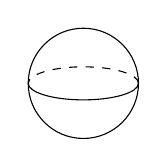
\begin{tikzpicture}[scale=.35]
						%\shade[ball color = gray!40, opacity = 0.4] (0,0) circle (2cm);
						\draw (0,0) circle (2cm);
						\draw (-2,0) arc (180:360:2 and 0.6);
						\draw[dashed] (2,0) arc (0:180:2 and 0.6);
						%\fill[fill=black] (0,0) circle (1pt);
					\end{tikzpicture}
				}
			\end{minipage}
			\vfill
			\bigskip
			\item<+-> Torus
			\begin{minipage}{2cm}
				\centering
				\resizebox{2cm}{!}{
					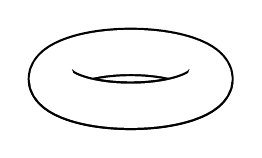
\begin{tikzpicture}[scale=.8,thick]
						\pic{torus={1cm}{2.8mm}{70}};
					\end{tikzpicture}
				}
			\end{minipage}
			\vfill
			\bigskip
			\item<+-> $S_{0,3}$: the sphere with $3$ punctures.
			\begin{minipage}{2cm}
				\resizebox{2cm}{!}{
					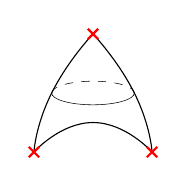
\begin{tikzpicture}[scale=.75]
						\draw[thin] plot[smooth,tension=1] coordinates {(-1,0) (-0.7,1) (0,2)};
						\draw[thin] plot[smooth,tension=1] coordinates {(1,0) (0.7,1) (0,2)};
						\draw[thin] plot[smooth,tension=1] coordinates {(-1,0) (0,.5) (1,0)};
						\node[cross out,draw,red, thick,scale=0.5] at (-1,0) {};
						\node[cross out,draw,red, thick,scale=0.5] at (1,0) {};
						\node[cross out,draw,red, thick,scale=0.5] at (0,2) {};
						\draw[very thin] (-.7,1) arc (180:360:.7 and .2);
						\draw[very thin, dashed] (-.7,1) arc (180:0:.7 and .2);
					\end{tikzpicture}
				}
			\end{minipage}
			\vfill
			\bigskip
			\item<+-> $\RP^2$: the set of all lines passing through the origin in $\R^3$.
			\begin{itemize}
				\item<+-> A basis for the topology in $\RP^2$ is the sets of lines that form a bounded angle from a fixed line $\ell$ in $\R^3$.
				%\item<+-> \textbf{Fact:} $\RP^2$ is a $2$-manifold.
			\end{itemize}
		\end{itemize}
	\end{frame}
	
	\begin{comment}
		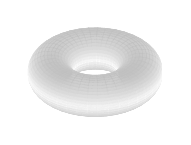
\begin{tikzpicture}[scale=.25]
			\begin{axis}[
				view={180}{60}, % Viewing angle
				hide axis, % Hide the axes
				samples=40, % Number of samples in the x direction
				samples y=40, % Number of samples in the y direction
				domain=0:360,
				y domain=0:360,
				z buffer=sort, % Improve 3D rendering
				]
				\addplot3[
				thin,
				surf,
				shader=flat mean,
				opacity=0.8, % Add some transparency
				mesh/rows=40, % Match the number of samples
				mesh/cols=40 % Match the number of samples y
				]
				(
				{(2 + cos(x)) * cos(y)}, 
				{(2 + cos(x)) * sin(y)}, 
				{sin(x)}
				);
			\end{axis}
		\end{tikzpicture}
	\end{comment}
	
	\begin{comment}
		\vfill
		\centering
		\begin{beamercolorbox}[sep=8pt,center,shadow=true,rounded=true]{title}
			\usebeamerfont{title}{How can we think of $\RP^2$?}\par%
		\end{beamercolorbox}
		\vfill
	\end{comment}
	%\section{How can we think of $\RP^2$?}
	
	\begin{frame}{Alternate View of $\RP^2$}
		\begin{definition}
			A \emph{plane} in $\R^3$ is a $2$-dimensional vector subspace of $\R^3$. An \emph{affine plane} $A$ is a translate of a plane $P$ by a nonzero vector $v$ that is not in $P$.
		\end{definition}
		\begin{center}
			\tdplotsetmaincoords{70}{110}
			\begin{tikzpicture}[scale=2,tdplot_main_coords]
				\def\x{1.5}
				\filldraw[draw=blue,fill=blue!20]          
				(-1,-1,0)
				-- (1,-1,0)
				-- (1,1,0)
				-- (-1,1,0)
				-- cycle;
				
				\filldraw[draw=red,fill=red!20]          
				(-.5,-.5,1)
				-- (1.5,-.5,1)
				-- (1.5,1.5,1)
				-- (-.5,1.5,1)
				-- cycle;
				
				\draw[black, -Stealth, circle] (0,0,0) -- (.5,.5,1) node[anchor=north east]{$v$};
				\filldraw[black] (.5,.5,1) circle(.25pt) node[above right] {};
				\draw[thick,-Stealth] (0,0,0) -- (\x,0,0) node[anchor=north east]{$x$};
				\draw[thick,-Stealth] (0,0,0) -- (0,\x,0) node[anchor=north east]{$y$};
				\draw[thick,-Stealth] (0,0,0) -- (0,0,\x) node[anchor=north east]{$z$};
				\draw (-.5, 1.5, 1) node[above right]{$A$};
				\draw (-1, 1, 0) node[above right]{$P$};
			\end{tikzpicture}	
		\end{center}

	\end{frame}
	
	\begin{frame}{Alternate View of $\RP^2$}
		\begin{lemma}
			Let $P$ be a plane passing through the origin in $\R^3$ and let $A$ be an affine plane which is a translate of $P$ by a nonzero vector $v$ not in $P$. Then,
			\begin{equation*}
				\RP^2 \cong A \sqcup \projof{P}
			\end{equation*}
		\end{lemma}
			
			\textbf{Note:} $\projof{P}$ is the subset of $\RP^2$ of lines passing through the origin and contained in $P$.
		%\pause
		
		\begin{center}
			\tdplotsetmaincoords{70}{110}
			\begin{tikzpicture}[scale=2,tdplot_main_coords]
				\def\x{1.5}
				\filldraw[draw=blue,fill=blue!20]          
				(-1,-1,0)
				-- (1,-1,0)
				-- (1,1,0)
				-- (-1,1,0)
				-- cycle;
				
				\filldraw[draw=red,fill=red!20]          
				(-.5,-.5,1)
				-- (1.5,-.5,1)
				-- (1.5,1.5,1)
				-- (-.5,1.5,1)
				-- cycle;
				
				\draw[black, -Stealth, circle] (0,0,0) -- (.5,.5,1) node[anchor=north east]{$v$};
				\filldraw[black] (.5,.5,1) circle(.25pt) node[above right] {};
				\draw[thick,-Stealth] (0,0,0) -- (\x,0,0) node[anchor=north east]{$x$};
				\draw[thick,-Stealth] (0,0,0) -- (0,\x,0) node[anchor=north east]{$y$};
				\draw[thick,-Stealth] (0,0,0) -- (0,0,\x) node[anchor=north east]{$z$};
				\draw (-.5, 1.5, 1) node[above right]{$A$};
				\draw (-1, 1, 0) node[above right]{$P$};
			\end{tikzpicture}	
		\end{center}
	\end{frame}
	
	\begin{comment}
		If lines is not contained in pi(P), it will intersect A at a single point we will then send the point in RP^2. If the line is contained in P, then we will send it to pi(P)
	\end{comment}
	
	% Last thing we need to review before moving on and starting to combine things togeht is the fundamental group
	\begin{frame}{Fundamental Groups}
		\begin{definition}
			Let $S$ be a path-connected a surface. For any point $p\in S$ the \emph{fundamental group} of $S$ is the set of equivalence classes (under homotopy) of the loops on $S$ based at $p$ with the concatenation operation. This group is denoted $\pi_1(S)$.
		\end{definition}
	\end{frame}
	\begin{comment}
		\begin{center}
			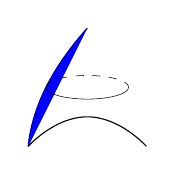
\begin{tikzpicture}[scale=.75]
				\draw[thin] plot[smooth,tension=1,name path=C] coordinates {(-1,0) (0,.5) (1,0)};
				%\node[cross out,draw,red, thick,scale=0.5] at (-1,0) {};
				%\node[cross out,draw,red, thick,scale=0.5] at (1,0) {};
				%\node[cross out,draw,red, thick,scale=0.5] at (0,2) {};
				\begin{scope}
					\draw[clip] plot[smooth,tension=1,name path=A] coordinates {(-1,0) (-0.7,1) (0,2)};
					\fill[blue] plot[smooth,tension=1,name path=B] coordinates {(1,0) (0.7,1) (0,2)} -- plot[smooth,tension=1,name path=A] coordinates {(-1,0) (-0.7,1) (0,2)};
				\end{scope}
				\draw[very thin] (-.7,1) arc (180:360:.7 and .2);
				\draw[very thin, dashed] (-.7,1) arc (180:0:.7 and .2);
			\end{tikzpicture}
		\end{center}
	\end{comment}
	
	\begin{frame}
		\begin{beamercolorbox}[sep=8pt,center,shadow=true,rounded=true]{title}
			\usebeamerfont{title}Questions?\par%
		\end{beamercolorbox}
		\begin{beamercolorbox}[sep=8pt,center,shadow=true,rounded=true]{title}
			\usebeamerfont{title}Hyperbolic Structures\par%
		\end{beamercolorbox}
	\end{frame}
	
	\begin{frame}{The Upper Half Plane}
		\begin{definition}
			The \emph{hyperbolic plane} $\Hyp^2$ is the metric space
			\begin{equation*}
				\Hyp^2 = \set{(x,y) \in \R^2 \colon y > 0} \qquad \metricd(u,v) = \inf_{u \to v} \int_0^1 \frac{\sqrt{\derof{x}(t)^2 + \derof{y}(t)^2}}{y(t)} \der{t}
			\end{equation*}
		\end{definition}			
		\begin{center}
			\begin{tikzpicture}[scale=.7]
				\begin{axis}[
					axis lines=middle,
					x axis line style={Stealth-Stealth, very thick},
					y axis line style={-{Stealth},very thick},
					xmin=-1.5, xmax=1.5, ymin=0, ymax=2.5,
					xlabel style={at={(axis description cs:1.04,0.04)},anchor=north},
					ylabel style={at={(axis description cs:0.45,1.04)},anchor=north},
					xlabel=$x$,
					ylabel=$y$,
					xticklabel=\empty,
					yticklabel=\empty,
					xtick=\empty,
					ytick=\empty]
					\addplot[domain=-.75:1.25,samples=400,blue,thick]{sqrt(1-(x-.25)^2)};
					\addplot+[only marks,mark=*,mark options={fill=black,black}, nodes near coords={$u$}] coordinates {(.3, 0.9987)};
					\addplot+[only marks,mark=*,mark options={fill=black,black}, nodes near coords={$v$}] coordinates {(1, 0.6614)};
				\end{axis}
			\end{tikzpicture}
		\end{center}
	\end{frame}
	
	% The upper half plane is a model of the hyperbolic plane where given two points u and v, the distance between u and v is the length ofthe shortest path beteween u and v. Our formula looks like the euclidean metric, but things that look close together near the x axis are really far apart. 
	
	\begin{frame}{Hyperbolic Structure on a Surface $S$}
		\begin{itemize}
			\item Every point $p \in S$ has a neighborhood that maps to an open subset of $\Hyp^2$
			\begin{center}
				\begin{multicols}{2}
					\begin{minipage}{0.5\textwidth}
						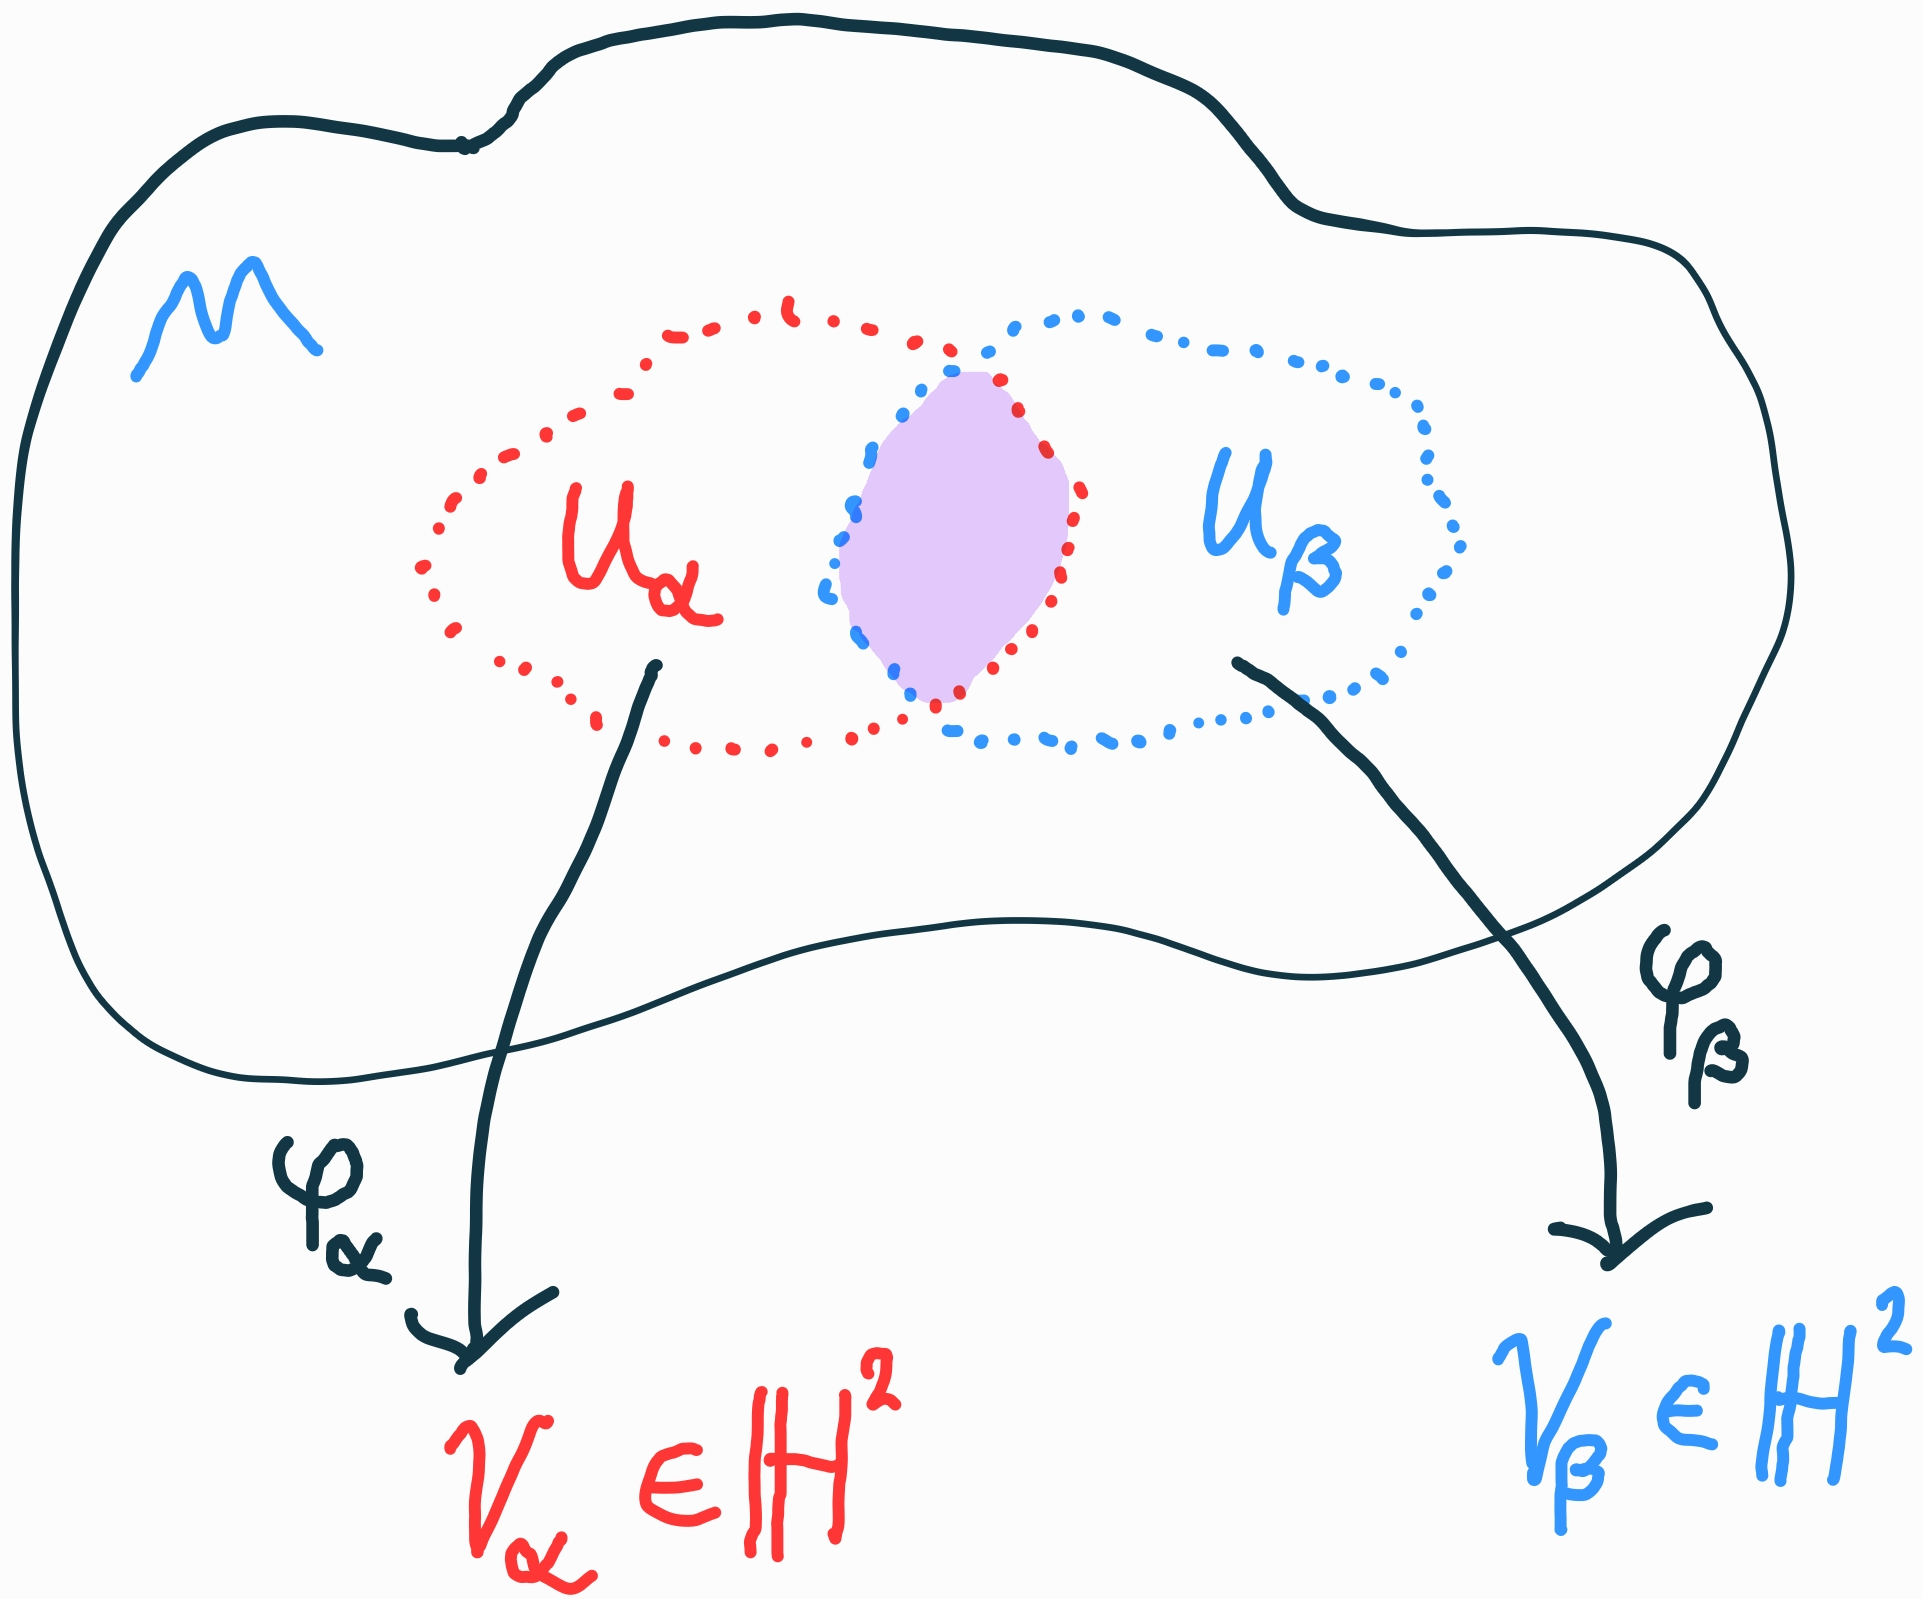
\includegraphics[width=\textwidth]{structure}
					\end{minipage}
					\begin{minipage}{0.5\textwidth}
						\begin{itemize}
							\item $\varphi_\alpha \colon U_\alpha \to V_\alpha$
							\item $\varphi_\beta \colon U_\beta \to V_\beta$
							\item $\restrict{\varphi_\beta \circ \varphi_\alpha}{\varphi_\alpha(U_\alpha) \cap \varphi_\beta(U_\beta)}$
							\item Needs to be isometry
						\end{itemize}
					\end{minipage}	
				\end{multicols}
			\end{center}
			\item This gives a notion of distance between two points on the surface $S$.
			\item Many surfaces have lots of hyperbolic structures, but \dots 
			\item $S_{0,3}$ only has one.
		\end{itemize}
	\end{frame}
	% hyperbolic structure says that each point in S
	\begin{frame}{The Hyperbolic Structure on $S_{0,3}$}
		\begin{minipage}{\linewidth}
			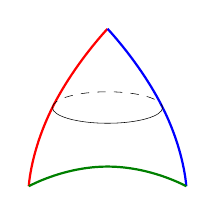
\begin{tikzpicture}[scale=1,baseline=(current bounding box.north)]
			\draw[thick,red] plot[smooth,tension=1] coordinates {(-1,0) (-0.7,1) (0,2)};
			\draw[thick,blue] plot[smooth,tension=1] coordinates {(1,0) (0.7,1) (0,2)};
			\draw[thick,darkgreen] plot[smooth,tension=1] coordinates {(-1,0) (0,.25) (1,0)};
			%\node[cross out,draw,red, thick,scale=0.5] at (-1,0) {};
			%\node[cross out,draw,red, thick,scale=0.5] at (1,0) {};
			%\node[cross out,draw,red, thick,scale=0.5] at (0,2) {};
			\draw[very thin] (-.7,1) arc (180:360:.7 and .2);
			\draw[very thin, dashed] (-.7,1) arc (180:0:.7 and .2);
			\end{tikzpicture}
			\qquad
			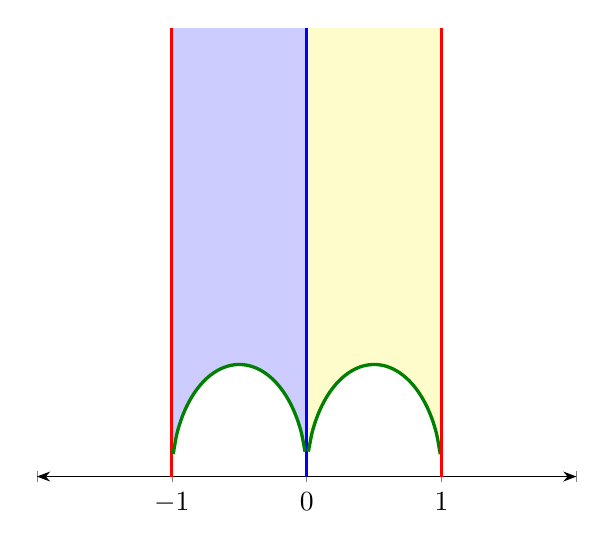
\begin{tikzpicture}[scale=1,baseline=(current bounding box.north)]
			\begin{axis}[
				axis lines=middle,
				x axis line style={Stealth-Stealth, thin},
				%y axis line style={-{Stealth},thin},
				xmin=-2, xmax=2, ymin=0, ymax=2,
				xticklabel=\empty,
				yticklabel=\empty,
				extra x ticks={-1,0,1},
				extra x tick labels={$-1$,0,$1$},
				ytick=\empty]
				\draw[red,very thick] (-1,0) -- (-1,2);
				\draw[blue,very thick] (0,0) -- (0,2);		
				\addplot+[smooth,samples=400,very thick,no marks,darkgreen,name path=A] {sqrt(.25-(x+.5)^2)}; % actual curve
				\addplot+[draw=none,no marks,name path=B] {2};     % “fictional” curve
				\addplot+[blue!20] fill between[of=A and B,soft clip={domain=-1:0}]; % fillin
				\addplot+[smooth,samples=400,very thick,no marks,darkgreen,name path=C] {sqrt(.25-(x-.5)^2)}; % actual curve
				\draw[red,very thick] (1,0) -- (1,2);
				\addplot+[draw=none,no marks,name path=D] {2};     % “fictional” curve
				\addplot+[yellow!20] fill between[of=C and D,soft clip={domain=0:1}];
				\draw[red,very thick] (1,0) -- (1,2);
			\end{axis}
			\end{tikzpicture}	
		\end{minipage}
	\end{frame}
	
	%\section{More Geometric Structures}
	
	\begin{frame}{Convex Real Projective Structures}
		\begin{definition}
			\begin{itemize}
				\item<+-> An open set $\Omega \subseteq \RP^2$ is \emph{proper} if there exists a plane $P \subseteq \R^3$ passing through the origin such that $\close{\Omega} \cap \projof{P} = \varnothing$.
				\item<+-> A proper set $\Omega \subseteq \RP^2$ is \emph{convex} if, for any two points $x,y \in \Omega$, the line $l_{xy}$ passing though $x$ and $y$ intersects $\Omega$ in a connected segment.
				\item<+-> $\Omega$ is \emph{strictly convex} if $\bound{\Omega}$ contains no straight line segments.
			\end{itemize}
		\end{definition}
		\onslide<3->{
			\begin{minipage}{\textwidth}
				\centering
				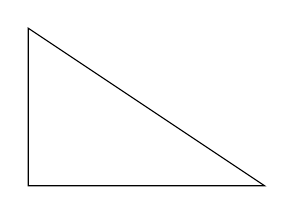
\begin{tikzpicture}
					\draw (0,0) -- (3,0) -- (0,2) -- cycle;
				\end{tikzpicture}
				\quad
				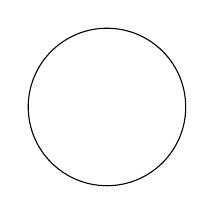
\begin{tikzpicture}
					\draw (0,0) circle (1);
				\end{tikzpicture}
				\quad
				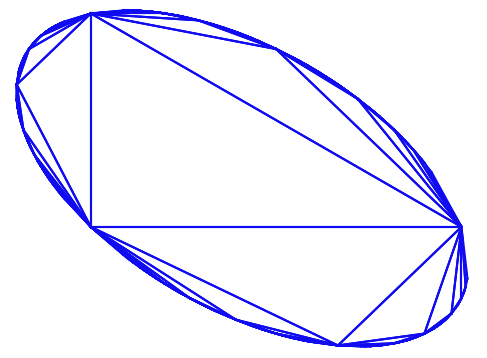
\includegraphics[width=0.25\textwidth]{strictly_convex_set_from_paper}
			\end{minipage}
		}
	\end{frame}
	
	\begin{frame}{Convex Real Projective Structures}
		Given a strictly convex set $\Omega$ in $\RP^2$.
		\begin{definition}
			The \emph{Hilbert distance} between any two distinct points $a,b \in \Omega$ is given by
			\begin{equation*}
				\metricd(a,b) =  \frac{1}{2} \log \CR{x,a,b,y}
			\end{equation*}
			\begin{center}
				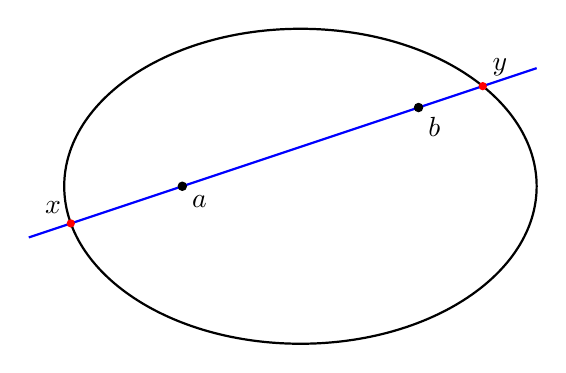
\begin{tikzpicture}
					\draw[thick,name path=line 1] (0,0) ellipse (3 and 2);
					\coordinate (a) at (-1.5,0);
					\coordinate (b) at (1.5,1);
					\node[below right] at (a) {$a$};
					\node[below right] at (b) {$b$};
					\draw[add= .65 and .5, blue, thick,name path=line 2] (a) to (b);
					\draw[fill=black] (a) circle (1.5pt);
					\draw[fill=black] (b) circle (1.5pt);
					\fill[red,name intersections={of=line 1 and line 2,total=\t}]
						\foreach \s in {1,...,\t}{(intersection-\s) circle (1.5pt)};
					\node[above left] at (intersection-2) {$x$};
					\node[above right] at (intersection-1) {$y$};
				\end{tikzpicture}	
			\end{center}
		\end{definition}
	\end{frame}
	
	\begin{frame}{Convex Real Projective Structures on $S_{0,3}$}
		\begin{itemize}
			\item<+-> Can equip $S_{0,3}$ with many convex real projective structures with their Hilbert metric%$(\RP^2, \PSL{3}{\R})$-structures
			\item<+-> Use reflections
			\begin{align*}
				R_{1,T} = 
				\begin{bmatrix}
					-1 & 0 & 0 \\
					2T & 1 & 0 \\
					\frac{2}{T} & 0 & 1
				\end{bmatrix} &
				\qquad R_{2,T} = 
				\begin{bmatrix}
					1 & \frac{2}{T} & 0 \\
					0 & -1 & 0 \\
					0 & 2T & 1
				\end{bmatrix} \\
				R_{3,T} = 
				\begin{bmatrix}
					1 & 0 & 2T \\
					0 & 1 & \frac{2}{T} \\
					0 & 0 & -1
				\end{bmatrix} &
			\end{align*}
			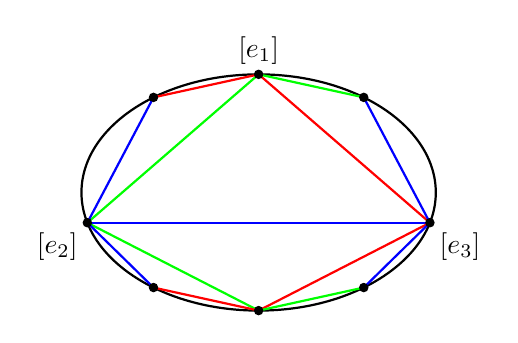
\begin{tikzpicture}[
				scale=1.5,
				R1_edge/.style={blue, thick},
				R2_edge/.style={red, thick},
				R3_edge/.style={green, thick}
				]
				\coordinate (e1) at (0,1);
				\coordinate (e2) at (-1.45,-0.25604);
				\coordinate (e3) at (1.45,-0.25604);
				\coordinate (R1e1) at (0,-1);
				\coordinate (R1R2e1) at (-.89,-0.80496);
				\coordinate (R1R3e1) at (.89,-0.80496);
				
				\coordinate (R2e2) at (.89,0.80496);
				\coordinate (R3e3) at (-.89,0.80496);
				
				\draw[thick] (0,0) ellipse (1.5cm and 1cm);
				\node[above] (pe1) at (e1) {$[e_1]$};
				\node[below left] (pe2) at (e2) {$[e_2]$};
				\node[below right] (pe3) at (e3) {$[e_3]$};
				
				\draw[R1_edge] (e2) -- (e3);
				\draw[R2_edge] (e1) -- (e3);
				\draw[R3_edge] (e1) -- (e2);
				
				\draw[R3_edge] (e2) -- (R1e1);
				\draw[R2_edge] (e3) -- (R1e1);

				\draw[R2_edge] (R1R2e1) -- (R1e1);
				\draw[R1_edge] (R1R2e1) -- (e2);
				\draw[R3_edge] (R1e1) -- (R1R3e1);
				\draw[R1_edge] (e3) -- (R1R3e1);
				
				\draw[R3_edge] (R2e2) -- (e1);
				\draw[R1_edge] (R2e2) -- (e3);
				
				\draw[R1_edge] (R3e3) -- (e2);
				\draw[R2_edge] (R3e3) -- (e1);
				
				\draw[fill=black,black] (e1) circle[radius=1pt];
				\draw[fill=black,black] (e3) circle[radius=1pt];
				\draw[fill=black,black] (e2) circle[radius=1pt];
				
				\draw[fill=black,black] (R1e1) circle[radius=1pt];
				\draw[fill=black,black] (R1R2e1) circle[radius=1pt];
	    		\draw[fill=black,black] (R1R3e1) circle[radius=1pt];
	    		
	    		\draw[fill=black,black] (R2e2) circle[radius=1pt];
	    		\draw[fill=black,black] (R3e3) circle[radius=1pt];
			\end{tikzpicture}
			\item<+-> There is a unique convex projective structure for every value of $T$.
			\item<+-> The hyperbolic structure corresponds to $T=1$.
		\end{itemize}
	\end{frame}
		%want to measure the similarities between these structures that capures the complexity of our convext real projective structure (numerical invarient)
	\begin{frame}{Hilbert Entropy}
		%\hl{Discuss how the matrices in the previous slide }
		\begin{definition}
			Let $\Omega$ be a convex real projective structure on a surface $S$ and $p \in \Omega$ be a fixed point. The Hilbert \emph{entropy} is given by
			\begin{equation*}
				h_\Omega = \lim_{x \to \infty} \frac{1}{x} \log \#\set{\gamma \in \pi_1(S_{0,3}) \colon \metricd_\Omega(p,\rho_T(\gamma)p) \leq x}
			\end{equation*}
			\begin{itemize}
				\item $\rho_T \colon \pi_1(S_{0,3}) \to \PSL{3}{\R}$ % make slidess	
			\end{itemize}
		\end{definition}
	\end{frame}
	
	\begin{frame}{The Manhattan Curve}
		\begin{itemize}
			\item<+-> The \emph{Manhattan Curve} is a way use the entropy to compare two convex projective structures.
		\end{itemize}
		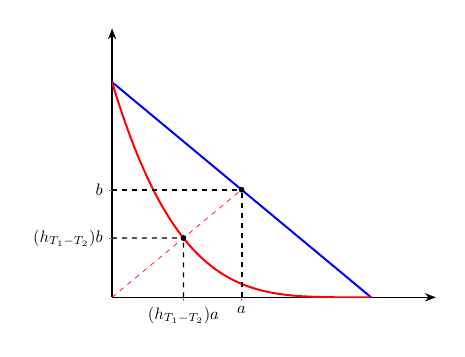
\begin{tikzpicture}[scale=.6]
			\newcommand{\pointa}{.5}
			\newcommand{\pointb}{.5}
			\newcommand{\ha}{0.27551}
			\newcommand{\hb}{0.27551}
			\begin{axis}[
				axis lines=middle,
				x axis line style={-{Stealth}, thick},
				y axis line style={-{Stealth},thick},
				xmin=0, xmax=1.25, ymin=0, ymax=1.25,
				xticklabel=\empty,
				yticklabel=\empty,
				ytick=\empty,
				xtick=\empty,
				extra x ticks={\ha,\pointa},
				extra x tick labels={$(h_{T_1-T_2})a$,$a$},
				extra y ticks={\hb,\pointb},
				extra y tick labels={$(h_{T_1-T_2})b$,$b$}
				]
				\addplot[domain=0:1,samples=5,blue,very thick]{-x+1};
				\addplot[smooth,domain=0:1,samples=100,red,very thick,name path=thecurve]{(x-1)^4};
				\coordinate (ab) at (\pointa,\pointb);
				\coordinate (hpoint) at (\ha,\hb);
				\draw[black,very thick,dashed] (\pointa,0) -- (ab);
				\draw[black,very thick,dashed] (0,\pointb) -- (ab);
				\draw[black,fill=black] (ab) circle (1.5pt);
				\draw[thin,red,dashed,name path=abline] (0,0) -- (ab);
				\fill[red,name intersections={of=abline and thecurve,total=\t}]
					\foreach \s in {1,...,\t}{(intersection-\s) circle (1.5pt)};
				\draw[black,fill=black] (intersection-1) circle (1.5pt);
				\draw[black,thick,dashed] (\ha,0) -- (intersection-1);
				\draw[black,thick,dashed] (0,\hb) -- (intersection-1);
			\end{axis}
		\end{tikzpicture}
		\raisebox{15ex}{
			\begin{minipage}{.4\textwidth}
				\begin{itemize}
					\item $a+b=1$
					\item $h_{T_1 - T_2}(a+b)$ 
				\end{itemize}
			\end{minipage}
		}
	\end{frame}
	
	\begin{frame}{Properties of The Manhattan Curve}
		\begin{itemize}
			\item<+-> Strictly convex
			\item<+-> Real analytic
		\end{itemize}
	\end{frame}
	
	\begin{frame}{Code to Estimate Entropy}
		\pause
		Goals:
		\begin{itemize}
			\item<+-> Generate a lot of group elements
			\item<+-> Store their singular values
				\begin{itemize}
					\item The singular values are related to the quantity $\metricd^H(p,\rho(\gamma))$
				\end{itemize}
			\item<+-> Estimate entropy
		\end{itemize}
	\end{frame}
	
	\begin{frame}{Structure of Reflection Group}
		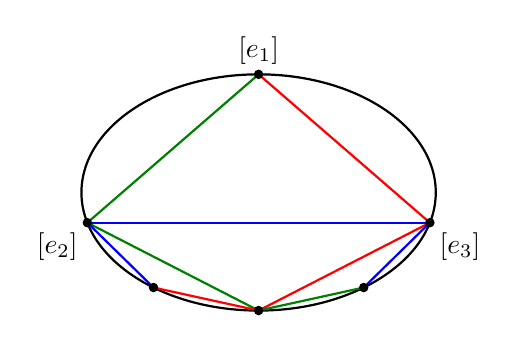
\begin{tikzpicture}[
			scale=1.5,
			R1_edge/.style={blue, thick},
			R2_edge/.style={red, thick},
			R3_edge/.style={darkgreen, thick}
			]
			
			\newcommand{\eone}{(0,1)}
			\newcommand{\etwo}{(-1.45,-0.25604)}
			\newcommand{\ethree}{(1.45,-0.25604)}
			\newcommand{\tone}{(0,-1)}
			\newcommand{\ttwo}{(-.89,-0.80496)}
			\newcommand{\tthree}{(.89,-0.80496)}
			
			\draw[thick] (0,0) ellipse (1.5cm and 1cm);
			\node[above] (e1) at \eone {$[e_1]$};
			\node[below left] (e2) at \etwo {$[e_2]$};
			\node[below right] (e3) at \ethree {$[e_3]$};
			
			\draw[R1_edge] \etwo -- \ethree;
			\draw[R2_edge] \eone -- \ethree;
			\draw[R3_edge] \eone -- \etwo;
			\onslide<2->{
				\draw[R3_edge] \etwo -- \tone;
				\draw[R2_edge] \ethree -- \tone;
			}
			\onslide<3->{
				\draw[R2_edge] \ttwo -- \tone;
				\draw[R1_edge] \ttwo -- \etwo;
			}
			\onslide<4->{
				\draw[R3_edge] \tone -- \tthree;
				\draw[R1_edge] \ethree -- \tthree;
			}
			
			\draw[fill=black,black] \eone circle[radius=1pt];
			\draw[fill=black,black] \ethree circle[radius=1pt];
			\draw[fill=black,black] \etwo circle[radius=1pt];
			
			\onslide<2->{\draw[fill=black,black] \tone circle[radius=1pt];}
			\onslide<3->{\draw[fill=black,black] \ttwo circle[radius=1pt];}
			\onslide<4->{\draw[fill=black,black] \tthree circle[radius=1pt];}
		\end{tikzpicture}
		\quad
		\onslide<5->{	
			\begin{tikzpicture}[
				R1_edge/.style={blue, thick},
				R2_edge/.style={red, thick},
				R3_edge/.style={darkgreen, thick},
				my_node/.style={black},
				level 1/.style = { level distance   = 10mm,
					sibling distance = 20mm },
				level 2/.style = { level distance   = 10mm,
					sibling distance = 20mm },
				level 3/.style = { level distance   = 10mm,
					sibling distance = 10mm }
				]
				\centering
				\node[my_node] {$0$}
				child {node[my_node] {$1$} edge from parent [R1_edge]
					child {node[my_node] {$2$} edge from parent [R3_edge]
						child {node[my_node] {$4$} edge from parent [R1_edge]}
						child {node[my_node] {$5$} edge from parent [R2_edge]}}
					child {node[my_node] {$3$} edge from parent[R2_edge]
						child {node[my_node] {$6$} edge from parent [R3_edge]}
						child {node[my_node] {$7$} edge from parent [R1_edge]}}
				};
			\end{tikzpicture}
		}
	\end{frame}
	
	\begin{frame}{How the Code Works}
		\begin{itemize}
			\item<+-> Takes in parameters $T$ and a maximum depth for the layer tree.
			\item<+-> Calculates the length of group element using the singular values.
			\item<+-> Counts number of elements who's lengths are in the interval $(n,n+1)$.
			\item<+-> Uses the count to calculate the approximate entropy.
		\end{itemize}
	\end{frame}
	
	\begin{frame}{Program Execution}
		\begin{center}
			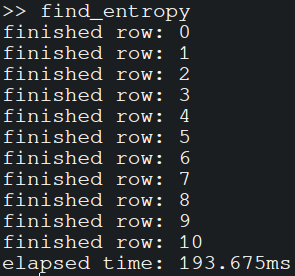
\includegraphics[width=.5\textwidth]{find_entropy_code}
			
\includegraphics[width=0.75\textwidth]{find_entropy_code_count}
		\end{center}
	\end{frame}
	
	\begin{frame}{Future Directions}
		\begin{itemize}
			\item<+-> Analyze symmetries of the Manhattan curve?
			\item<+-> Estimate the coordinates of the point where the slope of the tangent line of the Manhattan curve is equal to the slope of the secant line between the axes intercepts.
			\begin{itemize}
				\item<+-> Dynamical quantity called the \emph{correlation number}.
			\end{itemize}
			\item<+-> What happens to the Manhattan curve $\mathcal{M}(\rho_1, \rho_T)$ when $T$ gets large?
			\item<+-> Optimize code
			\item<+-> Generate more examples for different values of $T$.
		\end{itemize}
	\end{frame}
	
	\section{Thank You!}

\end{document}

